\documentclass{article}\usepackage[]{graphicx}\usepackage[]{color}
% maxwidth is the original width if it is less than linewidth
% otherwise use linewidth (to make sure the graphics do not exceed the margin)
\makeatletter
\def\maxwidth{ %
  \ifdim\Gin@nat@width>\linewidth
    \linewidth
  \else
    \Gin@nat@width
  \fi
}
\makeatother

\definecolor{fgcolor}{rgb}{0.345, 0.345, 0.345}
\newcommand{\hlnum}[1]{\textcolor[rgb]{0.686,0.059,0.569}{#1}}%
\newcommand{\hlstr}[1]{\textcolor[rgb]{0.192,0.494,0.8}{#1}}%
\newcommand{\hlcom}[1]{\textcolor[rgb]{0.678,0.584,0.686}{\textit{#1}}}%
\newcommand{\hlopt}[1]{\textcolor[rgb]{0,0,0}{#1}}%
\newcommand{\hlstd}[1]{\textcolor[rgb]{0.345,0.345,0.345}{#1}}%
\newcommand{\hlkwa}[1]{\textcolor[rgb]{0.161,0.373,0.58}{\textbf{#1}}}%
\newcommand{\hlkwb}[1]{\textcolor[rgb]{0.69,0.353,0.396}{#1}}%
\newcommand{\hlkwc}[1]{\textcolor[rgb]{0.333,0.667,0.333}{#1}}%
\newcommand{\hlkwd}[1]{\textcolor[rgb]{0.737,0.353,0.396}{\textbf{#1}}}%
\let\hlipl\hlkwb

\usepackage{framed}
\makeatletter
\newenvironment{kframe}{%
 \def\at@end@of@kframe{}%
 \ifinner\ifhmode%
  \def\at@end@of@kframe{\end{minipage}}%
  \begin{minipage}{\columnwidth}%
 \fi\fi%
 \def\FrameCommand##1{\hskip\@totalleftmargin \hskip-\fboxsep
 \colorbox{shadecolor}{##1}\hskip-\fboxsep
     % There is no \\@totalrightmargin, so:
     \hskip-\linewidth \hskip-\@totalleftmargin \hskip\columnwidth}%
 \MakeFramed {\advance\hsize-\width
   \@totalleftmargin\z@ \linewidth\hsize
   \@setminipage}}%
 {\par\unskip\endMakeFramed%
 \at@end@of@kframe}
\makeatother

\definecolor{shadecolor}{rgb}{.97, .97, .97}
\definecolor{messagecolor}{rgb}{0, 0, 0}
\definecolor{warningcolor}{rgb}{1, 0, 1}
\definecolor{errorcolor}{rgb}{1, 0, 0}
\newenvironment{knitrout}{}{} % an empty environment to be redefined in TeX

\usepackage{alltt}
\usepackage{amsmath}
\usepackage[margin=1in]{geometry}
\IfFileExists{upquote.sty}{\usepackage{upquote}}{}
\begin{document}

\section{Models}

\subsection{SVMALD}

\begin{align}
    \begin{bmatrix} Y_{1,t + 1} - Y_{1,t} \\ Y_{2,t + 1} - Y_{1,t} \\ V_{1,t + 1} - V_{1,t} \\ V_{2,t + 1} - V_{2,t} \end{bmatrix} = \begin{bmatrix} \mu_1 \Delta \\ \mu_2 \Delta \\ \kappa_1(\theta_1 - V_{1,t}) \Delta \\ \kappa_2(\theta_2 - V_{2,t}) \Delta \end{bmatrix} + \sqrt{\Delta}\Sigma_t^{\frac{1}{2}} \begin{bmatrix} \epsilon_{y_1,t+1} \\ \epsilon_{y_2,t+1} \\ \epsilon_{v_1,t+1} \\ \epsilon_{v_2,t+1} \end{bmatrix} + \begin{bmatrix} N_{t+1}(M_{y_1,t+1} \xi_{y_1, t+1} + M_{c,t+1} \xi_{y_1,c,t+1}) \\ N_{t+1}(M_{y_2,t+1} \xi_{y_2, t+1} + M_{c,t+1} \xi_{y_2,c,t+1}) \\ 0 \\ 0 \end{bmatrix}, \label{S_tdisc_2d}
\end{align}
where $\Sigma_{t} = \begin{bmatrix} V_{1,t} & \rho_y \sqrt{V_{1,t}V_{2,t}} & \rho_1 \sigma_{v,1} V_{1,t} & 0 \\ \rho_y \sqrt{V_{1,t}V_{2,t}} & V_{2,t} & 0 & \rho_2 \sigma_{v,2} V_{2,t} \\ \rho_1 \sigma_{v,1} V_{1,t} & 0 & \sigma_{v,1}^2 V_{1,t} & \rho_v \sigma_{v,1}\sigma_{v,2} \sqrt{V_{1,t} V_{2,t}} \\ 0 & \rho_2 \sigma_{v,2} V_{2,t} & \rho_v \sigma_{v,1}\sigma_{v,2} \sqrt{V_{1,t} V_{2,t}} & \sigma_{v,2}^2 V_{2,t} \end{bmatrix}$, \\$\epsilon_{k,t+1} \overset{iid}{\sim} N(0,1), k = \{y_1,y_2,v_1,v_2\}$, $\xi_{y_1,t+1} \overset{iid}{\sim} \mathcal{AL}_1(\mu_{y_1}, \nu_{y_1}^2)$, $\xi_{y_2,t+1} \overset{iid}{\sim} \mathcal{AL}_1(\mu_{y_2}, \nu_{y_2}^2)$, $\boldsymbol{\xi}_{c,t+1} = [\xi_{y_1,c,t+1}, \xi_{y_2,c,t+1}]' \overset{iid}{\sim} \mathcal{AL}_2(\boldsymbol{\mu}_c, \boldsymbol{\nu}_c)$, $\begin{bmatrix}
M_{y_1,t+1},M_{y_2,t+1},M_{c,t+1} \sim Multinomial(1;\frac{\lambda_{y_1}}{\lambda},\frac{\lambda_{y_2}}{\lambda},\frac{\lambda_c}{\lambda})
\end{bmatrix}$, and $N_{t+1} \sim Bernoulli(\lambda\Delta)$

\subsection{SVLD}

\begin{align}
    \begin{bmatrix} Y_{1,t + 1} - Y_{1,t} \\ Y_{2,t + 1} - Y_{1,t} \\ V_{1,t + 1} - V_{1,t} \\ V_{2,t + 1} - V_{2,t} \end{bmatrix} = \begin{bmatrix} \mu_1 \Delta \\ \mu_2 \Delta \\ \kappa_1(\theta_1 - V_{1,t}) \Delta \\ \kappa_2(\theta_2 - V_{2,t}) \Delta \end{bmatrix} + \sqrt{\Delta}\Sigma_t^{\frac{1}{2}} \begin{bmatrix} \epsilon_{y_1,t+1} \\ \epsilon_{y_2,t+1} \\ \epsilon_{v_1,t+1} \\ \epsilon_{v_2,t+1} \end{bmatrix} + \begin{bmatrix} N_{t+1}(M_{y_1,t+1} \xi_{y_1, t+1} ) \\ N_{t+1}(M_{y_2,t+1} \xi_{y_2, t+1} ) \\ 0 \\ 0 \end{bmatrix}, \label{S_tdisc_2d}
\end{align}
where $\Sigma_{t} = \begin{bmatrix} V_{1,t} & \rho_y \sqrt{V_{1,t}V_{2,t}} & \rho_1 \sigma_{v,1} V_{1,t} & 0 \\ \rho_y \sqrt{V_{1,t}V_{2,t}} & V_{2,t} & 0 & \rho_2 \sigma_{v,2} V_{2,t} \\ \rho_1 \sigma_{v,1} V_{1,t} & 0 & \sigma_{v,1}^2 V_{1,t} & \rho_v \sigma_{v,1}\sigma_{v,2} \sqrt{V_{1,t} V_{2,t}} \\ 0 & \rho_2 \sigma_{v,2} V_{2,t} & \rho_v \sigma_{v,1}\sigma_{v,2} \sqrt{V_{1,t} V_{2,t}} & \sigma_{v,2}^2 V_{2,t} \end{bmatrix}$, \\$\epsilon_{k,t+1} \overset{iid}{\sim} N(0,1), k = \{y_1,y_2,v_1,v_2\}$, $\xi_{y_1,t+1} \overset{iid}{\sim} \mathcal{AL}_1(0, \nu_{y_1}^2)$, $\xi_{y_2,t+1} \overset{iid}{\sim} \mathcal{AL}_1(0, \nu_{y_2}^2)$, $\begin{bmatrix}
M_{y_1,t+1},M_{y_2,t+1},M_{c,t+1} \sim Multinomial(1;\frac{\lambda_{y_1}}{\lambda},\frac{\lambda_{y_2}}{\lambda},\frac{\lambda_c}{\lambda})
\end{bmatrix}$, and $N_{t+1} \sim Bernoulli(\lambda\Delta)$

\subsection{SVMVN}

\begin{align}
    \begin{bmatrix} Y_{1,t + 1} - Y_{1,t} \\ Y_{2,t + 1} - Y_{1,t} \\ V_{1,t + 1} - V_{1,t} \\ V_{2,t + 1} - V_{2,t} \end{bmatrix} = \begin{bmatrix} \mu_1 \Delta \\ \mu_2 \Delta \\ \kappa_1(\theta_1 - V_{1,t}) \Delta \\ \kappa_2(\theta_2 - V_{2,t}) \Delta \end{bmatrix} + \sqrt{\Delta}\Sigma_t^{\frac{1}{2}} \begin{bmatrix} \epsilon_{y_1,t+1} \\ \epsilon_{y_2,t+1} \\ \epsilon_{v_1,t+1} \\ \epsilon_{v_2,t+1} \end{bmatrix} + \begin{bmatrix} N_{t+1}(M_{y_1,t+1} \xi_{y_1, t+1} + M_{c,t+1} \xi_{y_1,c,t+1}) \\ N_{t+1}(M_{y_2,t+1} \xi_{y_2, t+1} + M_{c,t+1} \xi_{y_2,c,t+1}) \\ 0 \\ 0 \end{bmatrix}, \label{S_tdisc_2d}
\end{align}
where $\Sigma_{t} = \begin{bmatrix} V_{1,t} & \rho_y \sqrt{V_{1,t}V_{2,t}} & \rho_1 \sigma_{v,1} V_{1,t} & 0 \\ \rho_y \sqrt{V_{1,t}V_{2,t}} & V_{2,t} & 0 & \rho_2 \sigma_{v,2} V_{2,t} \\ \rho_1 \sigma_{v,1} V_{1,t} & 0 & \sigma_{v,1}^2 V_{1,t} & \rho_v \sigma_{v,1}\sigma_{v,2} \sqrt{V_{1,t} V_{2,t}} \\ 0 & \rho_2 \sigma_{v,2} V_{2,t} & \rho_v \sigma_{v,1}\sigma_{v,2} \sqrt{V_{1,t} V_{2,t}} & \sigma_{v,2}^2 V_{2,t} \end{bmatrix}$, \\$\epsilon_{k,t+1} \overset{iid}{\sim} N(0,1), k = \{y_1,y_2,v_1,v_2\}$, $\xi_{y_1,t+1} \overset{iid}{\sim} N(\mu_{y_1}, \nu_{y_1}^2)$, $\xi_{y_2,t+1} \overset{iid}{\sim} N(\mu_{y_2}, \nu_{y_2}^2)$, $\boldsymbol{\xi}_{c,t+1} = [\xi_{y_1,c,t+1}, \xi_{y_2,c,t+1}]' \overset{iid}{\sim} MVN(\boldsymbol{\mu}_c, \boldsymbol{\nu}_c)$, $\begin{bmatrix}
M_{y_1,t+1},M_{y_2,t+1},M_{c,t+1} \sim Multinomial(1;\frac{\lambda_{y_1}}{\lambda},\frac{\lambda_{y_2}}{\lambda},\frac{\lambda_c}{\lambda})
\end{bmatrix}$, and $N_{t+1} \sim Bernoulli(\lambda\Delta)$

\subsection{SVIND}
\begin{align}
    \begin{bmatrix} Y_{t+1} - Y_t \\ V_{t+1} - V_t \end{bmatrix} = \begin{bmatrix}\mu\Delta \\ \kappa(\theta - V_{t})\Delta\end{bmatrix}  + \sqrt{V_{t}\Delta} \begin{bmatrix} 1 & 0 \\ \rho \sigma_v & \sqrt{1 - \rho^2} \sigma_v \end{bmatrix} \begin{bmatrix} \epsilon_{y,t+1} \\ \epsilon_{v,t+1} \end{bmatrix} + \begin{bmatrix} N_{y,t+1} \xi_{y,t+1} \\0  \end{bmatrix}, \label{S_tdisc}
\end{align}

$\epsilon_{k,t+1} \overset{iid}{\sim} N(0,1), k = \{y,v\}$, $\xi_{y,t+1} \overset{iid}{\sim} \mathcal{AL}_1(\mu_y, \nu_y^2)$, $N_{y,t+1} \sim Bernoulli(\lambda\Delta)$

\newpage
\section{Empirical study: S\&P and BTC jointly}

\subsection{Results: Joint Jumps}
\begin{knitrout}
\definecolor{shadecolor}{rgb}{0.969, 0.969, 0.969}\color{fgcolor}\begin{kframe}


{\ttfamily\noindent\itshape\color{messagecolor}{\#\# \\\#\# Attaching package: 'dplyr'}}

{\ttfamily\noindent\itshape\color{messagecolor}{\#\# The following objects are masked from 'package:stats':\\\#\# \\\#\# \ \ \ \ filter, lag}}

{\ttfamily\noindent\itshape\color{messagecolor}{\#\# The following objects are masked from 'package:base':\\\#\# \\\#\# \ \ \ \ intersect, setdiff, setequal, union}}\begin{verbatim}
## List of 13
##  $ lambda  : num [1:4] 0.097 0.0367 0.085 0.7813
##  $ sigma_v : num [1:2] 0.436 0.212
##  $ sigma_c : num [1:2] 1.074 0.174
##  $ rhoc    : num -0.104
##  $ xi_cw   : num [1:2] -5.236 -0.166
##  $ xi_y1eta: num 0.839
##  $ xi_y1w  : num 4.91
##  $ xi_y2eta: num 0.347
##  $ xi_y2w  : num -0.668
##  $ phi     : num [1:2] 0.985 0.976
##  $ theta   : num [1:2] 6.96 1.12
##  $ mu      : num [1:2] 0.165 0.0547
##  $ rho     : num [1:4] 0.00665 0.07259 0.45863 -0.70195
\end{verbatim}
\end{kframe}
\end{knitrout}

\clearpage
\newpage

\begin{knitrout}
\definecolor{shadecolor}{rgb}{0.969, 0.969, 0.969}\color{fgcolor}\begin{kframe}
\begin{alltt}
\hlcom{#Related to joint jumps:}

\hlstd{keepsBTCSP}\hlopt{$}\hlstd{xi_cw} \hlopt
  \hlkwd{as.data.frame}\hlstd{()} \hlopt
  \hlkwd{melt}\hlstd{()} \hlopt
  \hlkwd{mutate}\hlstd{(}\hlkwc{variable} \hlstd{=} \hlkwd{factor}\hlstd{(variable,} \hlkwc{levels} \hlstd{=} \hlkwd{c}\hlstd{(}\hlstr{"V1"}\hlstd{,} \hlstr{"V2"}\hlstd{),}\hlkwc{labels} \hlstd{=} \hlkwd{c}\hlstd{(}\hlstr{"BTC"}\hlstd{,} \hlstr{"S&P"}\hlstd{)))}\hlopt
  \hlkwd{ggplot}\hlstd{()} \hlopt{+}
  \hlkwd{geom_histogram}\hlstd{(}\hlkwd{aes}\hlstd{(}\hlkwc{x} \hlstd{= value))} \hlopt{+}
  \hlkwd{facet_grid}\hlstd{(}\hlopt{~}\hlstd{variable)}\hlopt{+}
  \hlkwd{ggtitle}\hlstd{(}\hlstr{"w_c (location of MALD)"}\hlstd{)}
\end{alltt}


{\ttfamily\noindent\itshape\color{messagecolor}{\#\# No id variables; using all as measure variables}}

{\ttfamily\noindent\itshape\color{messagecolor}{\#\# `stat\_bin()` using `bins = 30`. Pick better value with `binwidth`.}}\end{kframe}
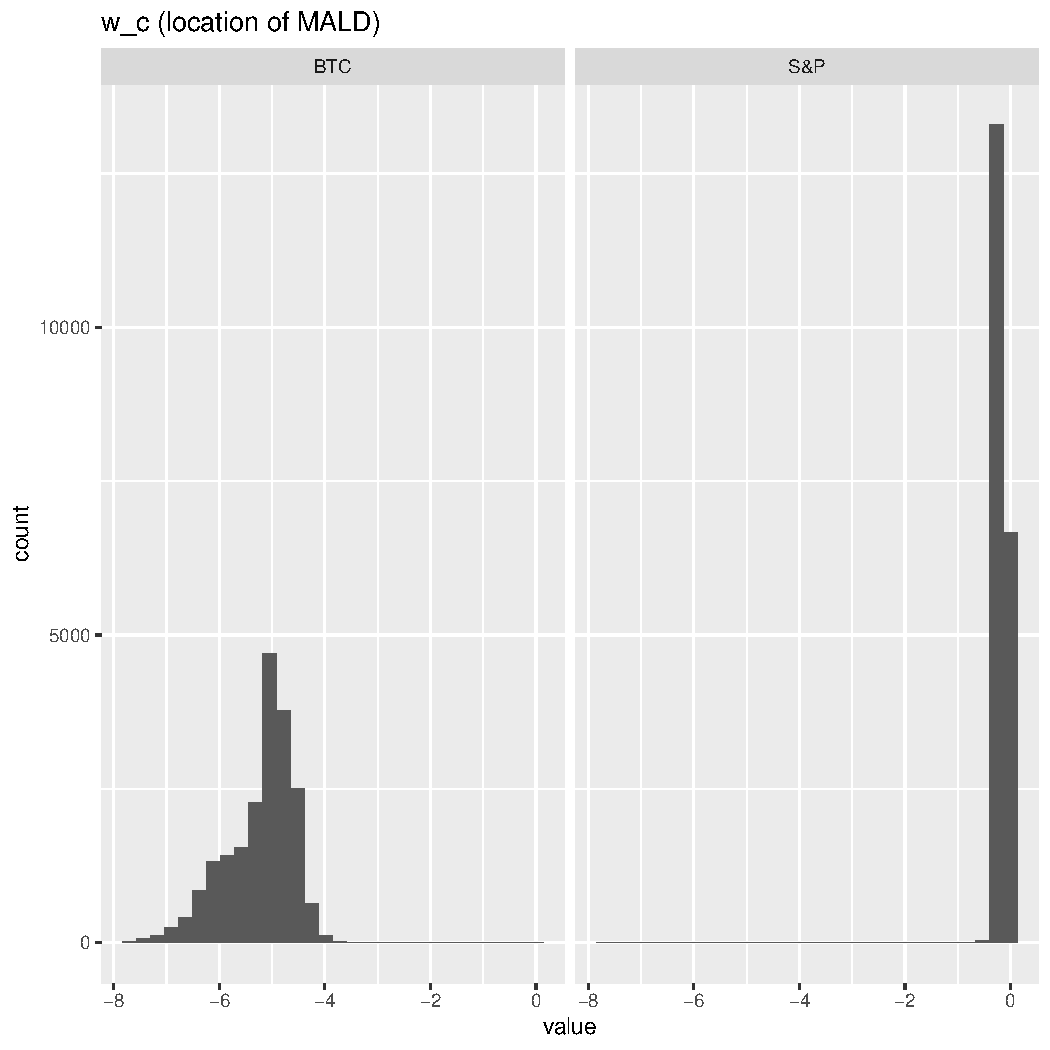
\includegraphics[width=6in,height=5in]{figure/unnamed-chunk-2-1} 
\end{knitrout}
\clearpage
\newpage



\begin{knitrout}
\definecolor{shadecolor}{rgb}{0.969, 0.969, 0.969}\color{fgcolor}\begin{kframe}
\begin{alltt}
\hlstd{keepsBTCSP}\hlopt{$}\hlstd{sigma_c} \hlopt
    \hlkwd{as.data.frame}\hlstd{()} \hlopt
  \hlkwd{melt}\hlstd{()} \hlopt
  \hlkwd{mutate}\hlstd{(}\hlkwc{variable} \hlstd{=} \hlkwd{factor}\hlstd{(variable,} \hlkwc{levels} \hlstd{=} \hlkwd{c}\hlstd{(}\hlstr{"V1"}\hlstd{,} \hlstr{"V2"}\hlstd{),}\hlkwc{labels} \hlstd{=} \hlkwd{c}\hlstd{(}\hlstr{"BTC"}\hlstd{,} \hlstr{"S&P"}\hlstd{)))}\hlopt
  \hlkwd{ggplot}\hlstd{()} \hlopt{+}
  \hlkwd{geom_histogram}\hlstd{(}\hlkwd{aes}\hlstd{(}\hlkwc{x} \hlstd{= value))} \hlopt{+}
  \hlkwd{facet_grid}\hlstd{(}\hlopt{~}\hlstd{variable)} \hlopt{+}
  \hlkwd{ggtitle}\hlstd{(}\hlstr{"sigma_c (scale of MALD)"}\hlstd{)}
\end{alltt}


{\ttfamily\noindent\itshape\color{messagecolor}{\#\# No id variables; using all as measure variables}}

{\ttfamily\noindent\itshape\color{messagecolor}{\#\# `stat\_bin()` using `bins = 30`. Pick better value with `binwidth`.}}\end{kframe}
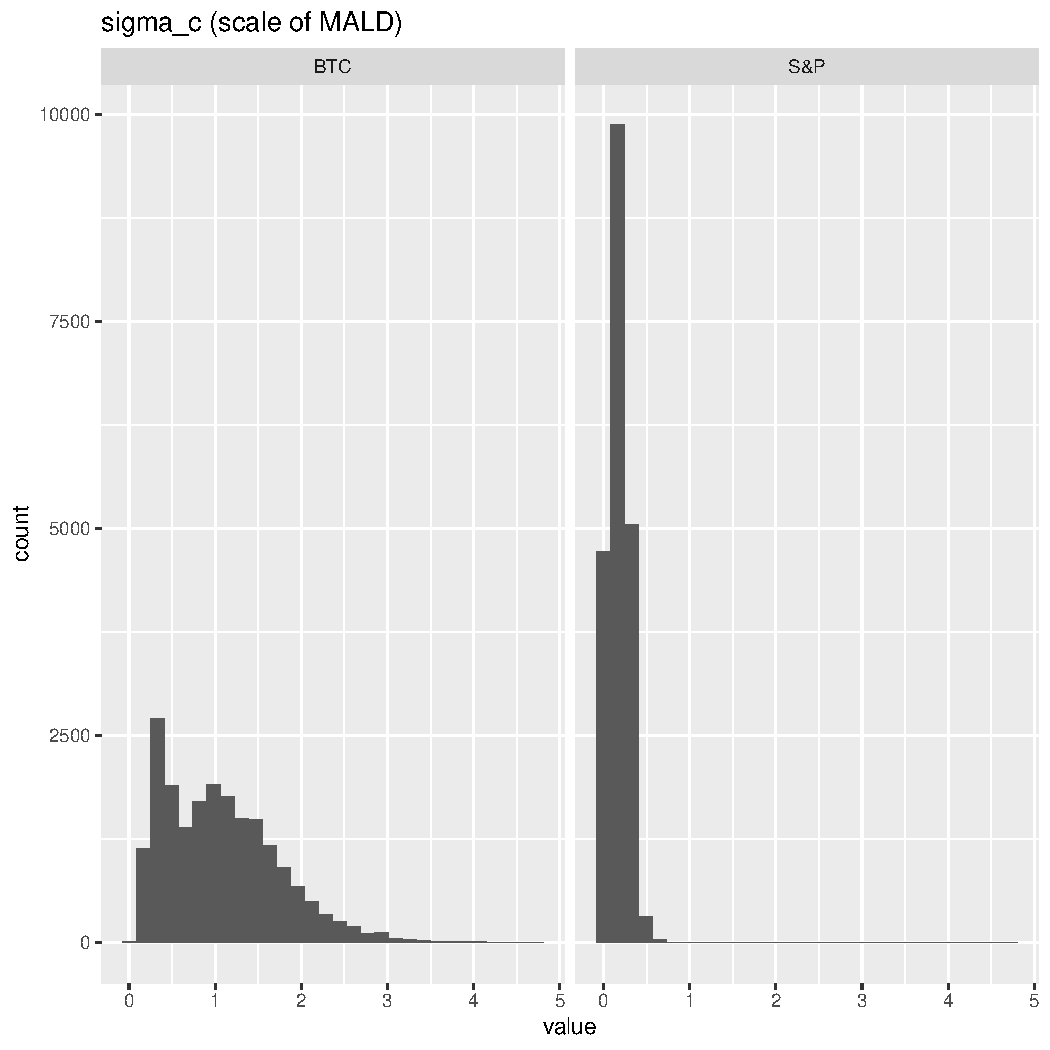
\includegraphics[width=6in,height=5in]{figure/unnamed-chunk-3-1} 
\end{knitrout}

\clearpage
\newpage

\begin{knitrout}
\definecolor{shadecolor}{rgb}{0.969, 0.969, 0.969}\color{fgcolor}\begin{kframe}
\begin{alltt}
  \hlkwd{ggplot}\hlstd{()} \hlopt{+}
  \hlkwd{geom_histogram}\hlstd{(}\hlkwd{aes}\hlstd{(}\hlkwc{x} \hlstd{= keepsBTCSP}\hlopt{$}\hlstd{rhoc))} \hlopt{+}
  \hlkwd{ggtitle}\hlstd{(}\hlstr{"rho_c (correlation of MALD)"}\hlstd{)}
\end{alltt}


{\ttfamily\noindent\itshape\color{messagecolor}{\#\# `stat\_bin()` using `bins = 30`. Pick better value with `binwidth`.}}\end{kframe}
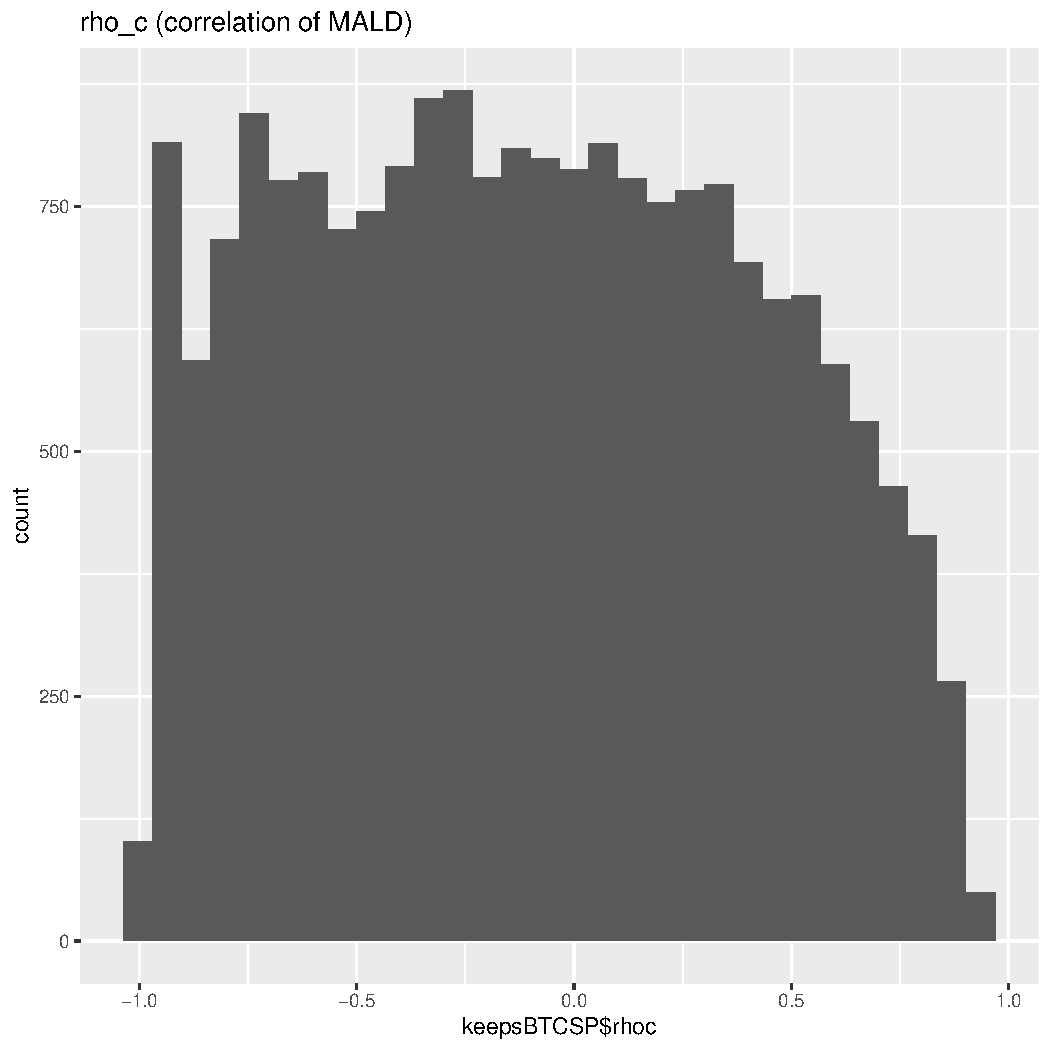
\includegraphics[width=5in,height=5in]{figure/unnamed-chunk-4-1} 
\end{knitrout}

\clearpage
\newpage

\begin{knitrout}
\definecolor{shadecolor}{rgb}{0.969, 0.969, 0.969}\color{fgcolor}\begin{kframe}
\begin{alltt}
\hlstd{keepsBTCSP}\hlopt{$}\hlstd{delta} \hlopt
  \hlkwd{melt}\hlstd{()} \hlopt
  \hlkwd{mutate}\hlstd{(}\hlkwc{value} \hlstd{=} \hlkwd{factor}\hlstd{(value,} \hlkwc{levels} \hlstd{=} \hlkwd{c}\hlstd{(}\hlnum{0}\hlopt{:}\hlnum{3}\hlstd{),}
                        \hlkwc{labels} \hlstd{=} \hlkwd{c}\hlstd{(}\hlstr{"BTC jump"}\hlstd{,} \hlstr{"S&P jump"}\hlstd{,} \hlstr{"Joint jump"}\hlstd{,} \hlstr{"No jump"}\hlstd{)))} \hlopt
  \hlkwd{ggplot}\hlstd{()} \hlopt{+}
  \hlkwd{geom_bar}\hlstd{(}\hlkwd{aes}\hlstd{(}\hlkwc{x} \hlstd{= Var2,} \hlkwc{fill} \hlstd{= value),} \hlkwc{position} \hlstd{=} \hlstr{"fill"}\hlstd{)} \hlopt{+}
  \hlkwd{scale_fill_brewer}\hlstd{(}\hlstr{"Type"}\hlstd{,}\hlkwc{type} \hlstd{=} \hlstr{"qual"}\hlstd{)} \hlopt{+}\hlkwd{labs}\hlstd{(}\hlkwc{x} \hlstd{=} \hlstr{"Time"}\hlstd{,} \hlkwc{y} \hlstd{=} \hlstr{"Proportion"}\hlstd{)}
\end{alltt}
\end{kframe}
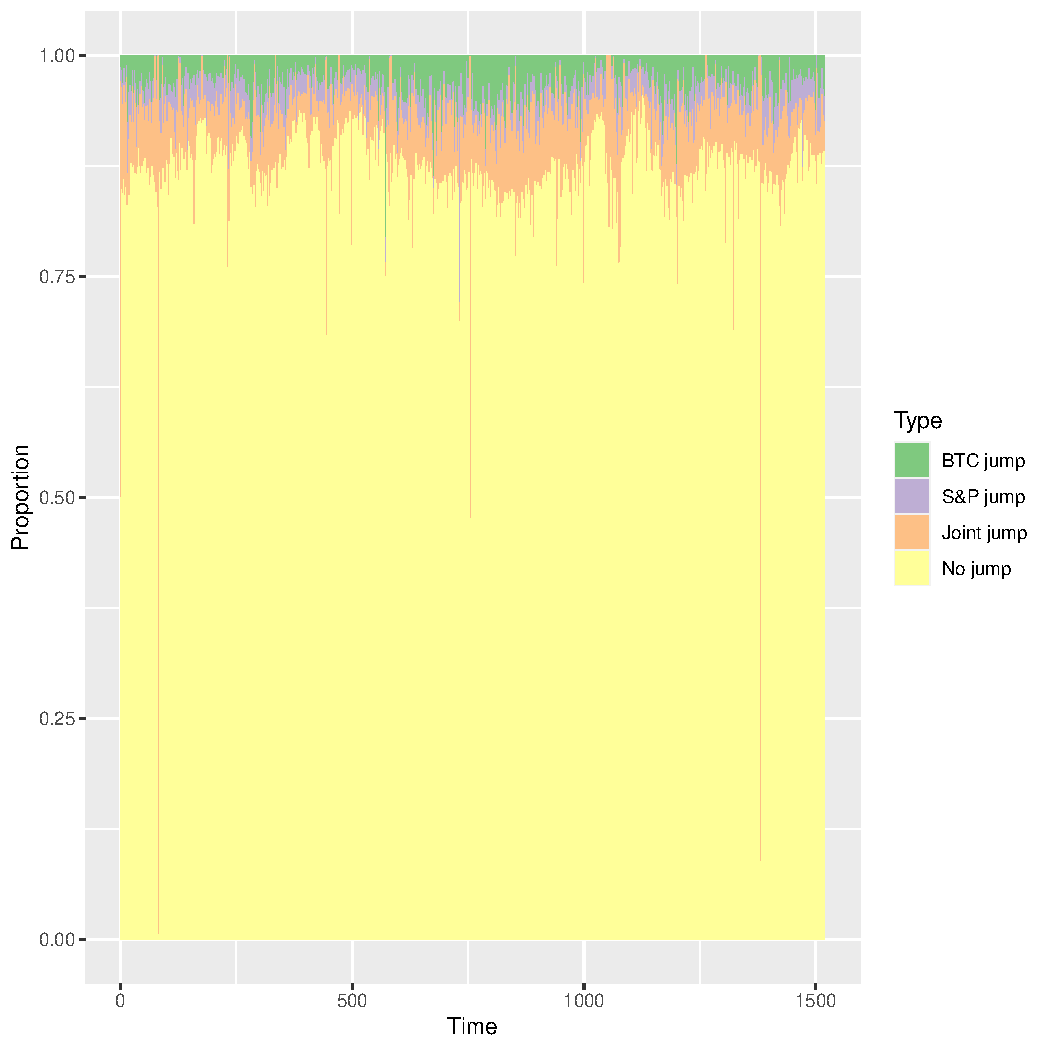
\includegraphics[width=6in,height=5in]{figure/unnamed-chunk-5-1} 
\begin{kframe}\begin{alltt}
\hlcom{#it's worth noting the MVN plot looks almost identical - same patterns}
\end{alltt}
\end{kframe}
\end{knitrout}


\clearpage
\newpage

\subsection{DIC}
 $$DIC_7 = -4E_{\theta,\boldsymbol{z} | \boldsymbol{y}}(ln(p(\boldsymbol{y}|\theta,\boldsymbol{z}))) + 2ln(p(\boldsymbol{y}|\hat{\theta}, \hat{\boldsymbol{z}})).$$ 
 
\begin{table}[]
\begin{tabular}{|l|l|l|l|l|}
\hline
                   & SVMALD  & SVLD    & SVMVN   & SVIND \\ \hline
Diffuse priors     &9813.312 &\textbf{9796.879} &9818.368 &10953.52 \\ \hline
Fulop-style priors &9827.731 &9854.88 &\textbf{9714.333} &10884.23 \\ \hline
\end{tabular}
\caption{\label{tab:dic7} Resulting DIC from runs with diffuse priors and runs with more informative priors. }
\end{table}
 

\subsection{Posterior predictive p-values}

First, a lineup to motivate. Posterior predictive p-values operate on the assumption that $p(y^* \mid Y) = \int p(y^* \mid \theta)p(\theta \mid Y) d \theta$ should be consistent with what we observed in $Y$.

\includegraphics[width = .9\linewidth]{"lineup_BTC.pdf"}

\newpage
\clearpage

\includegraphics[width = .9\linewidth]{"lineup_SP.pdf"}

\newpage
\clearpage

\includegraphics[width = .9\linewidth]{"ppp_joint_jumps.pdf"}

\end{document}
